\documentclass{article}
\usepackage[utf8]{inputenc}
\usepackage[english]{babel}
\usepackage[]{amsthm} %lets us use \begin{proof}
\usepackage[]{amssymb} %gives us the character \varnothing
\usepackage{mathtools}
\renewcommand{\qedsymbol}{\rule{0.7em}{0.7em}}
\usepackage{amsmath}
\usepackage{titlesec} 
\usepackage{float}

\titleformat{\section}[runin]
  {\normalfont\large\bfseries}{\thesection}{1em}{}
\titleformat{\subsection}[runin]
  {\normalfont\normalsize\bfseries}{\thesubsection}{1em}{}
\titleformat{\subsubsection}[runin]
  {\normalfont\normalsize\bfseries}{\thesubsubsection}{1em}{}

\newcommand{\Int}{\int\limits}


\title{Understanding the dynamics of a complex biological network without 
parameter information: Case study on the cell-cycle network 
of fission-yeast (\textit{S.pombe})}
\author{Souvadra Hati (Sr: 15551)}
\date\today
%This information doesn't actually show up on your document unless you use the maketitle command below

\begin{document}
\maketitle %This command prints the title based on information entered above

%Section and subsection automatically number unless you put the asterisk next to them.
% ************************************************************************* %
%                              Introduction                                 %
% ************************************************************************* %
\section*{Introduction:} Understanding and predicting the dynamics of complex 
biochemical networks is one of the fundamental goal of Systems Biology. Although,
even a single cell is way too complex in nature for us to model all its 
biochemical behaviours using our current understanding and compute capacity,
scientists have been successful in modelling some of the biochemical pathways
essentials in every living organism. One of the computationally feasible ways 
to predict the dynamical behaviours of these networks is to numerically solve a bunch of 
coupled Ordinary Differential Equations (ODEs) with appropriate kinetic parameters 
that can be experimentally measured. But that process requires extensive wet-lab
experiments to find out the vast array of biochemical parameters necessary to 
model even modests of the biological pathways, which slows down the process of 
building the models. This has motivated scientists to come up with innovative 
ideas to be able to gain insight into a biochemical pathway without extensive 
knowledge of the parameters involved in it. In this article I am going to discuss
two such ways of modelling a network and show how they can be useful by applying 
them in the cell-cycle pathway of fission-yeast (\textit{S.pombe}).
% ************************************************************************* %
%                             Discrete Method                               %
% ************************************************************************* %
\section*{Discrete Method:}
One of the most simple yet elegant way to model the essentials of a network is
to model it as a graph model with each protein / regulator can be assumed as 
a node and the interaction between those regulators as the edges of the graph.
The edges will only represent the the sign of the relation between those two nodes.
What I mean, is that the node will only take into account of the fact that 
the interaction is activating (+1) or inhibiting (-1). After that, in each 
discrete ieration the state of the the daughter nodes of the initialized nodes 
(can be themselves as well if self-activation or self-inhibition is present)
will be updated as per the update rule mentioned below.

\begin{equation*}
  S_i (t+1) = \begin{cases}
    0, & \text{if } \sum_{j} a_{ij} S_j(t) < \theta_i\\
    1, & \text{if } \sum_{j} a_{ij} S_j(t) > \theta_i\\
    S_i (t), & \text{if } \sum_{j} a_{ij} S_j(t) = \theta_i
    \end{cases}
\end{equation*}
Here, $S_j(t) \in \{0,1\}$ in the binary value assigned to node $j$ at iteration
$t$, which discretely denotes if the protein is present in the system at that 
iteration or not. $a_{ij} = 1$ denotes an activating interaction from node j to 
node i, and similarly $a_{ij}$ denotes an inhibiting edge and $a_{ij} = 0$
denotes no interaction (no edge between those two nodes). $\theta_{ij}$ is a 
threshold of activation of node $i$ which is generally $0$, unless otherwise 
mentioned \cite{boolean_model}.

One interesting aspect of this Boolean modelling is that, we can actually 
start the model iteration using all the possible initial conditions and that 
will be in most cases very much computationally feasible. For example, if our 
network of interest has 7 nodes, then there will be in total $2^7 = 128$, which 
means we can effectively sample the total solution space of the network which 
is absolutely not possible in a continuous scenario.

So, in this manner, without any knowledge of the kinetic parameters in the model
or ever solving any ODE at all, we can gain insight into the dynamics of the model
as I shall discuss using a case study in the later half of the report.
% ************************************************************************* %
%                           Continuous Method                               %
% ************************************************************************* %
\section*{Continuous Method:} Although the discrete method in theory can provide
us a lot of information regarding the network of interest, the harsh reality 
is that no biological system is actually discrete and introducing even moderate
amount of realism requires us to write the ODE of the reaction kinetics and solve 
them numerically to observe the dynamics of the network. But that requires 
access to the set of kinetic parameters that we are trying to avoid in our 
modelling paradigm. 

So, to tackle that exact challenge Huang et al. 2018 \cite{RACIPE} published 
an article on a software that they named ``RACIPE: Random Circuit Perturbation".
It takes, just like the Boolean method, only the topology of the core regulatory
circuit and unbiasly generates an ensemble of mathematical models, each of which 
is characterized by a unique set of kinetic parameters From the ensemble of 
models, we can analyze the robust dynamical properteis of the core circuit via 
downstream statistical analysis. In RACIPE, the effects of the "peripheral 
factors" are modeled as random perturbations to the kinetic parameters. RACIPE
samples its parameters across a wide range (via some random distribution) 
keeping the half functional rule (
which states that each regulatory link has about $50\%$ chance to be activated)
valid. The RACIPE generated gene-expression data can later be analyzed using 
differnt statistical tools (primarily Hierarchical clustering analysis (HCA), 
and Principal Component Analysis (PCA)) to get a holistic view of the dynamical 
feature of the network. All these are based of the previous studies that says 
that robust features in any gene regulatory network remains conserved against
large parameter purturbations due to the the restraints from the circuit 
topology itself. 

\begin{figure}[H]
  \centering
  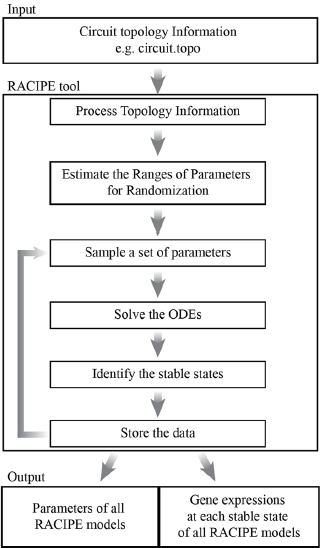
\includegraphics[width=70mm, scale=0.5]{racipe_workflow.png} \\
  \text{Figure 1: Workflow of RACIPE \cite{RACIPE}}
\end{figure}

\subsubsection*{Input:} The primary input of this toolbox is the circuit
topology that is written in a `.topo' file (e.g. ``circuit.topo"). Each line 
of this file specifies a regulatory link, which contains the source node, 
target node and mode of interaction (1 for activation, 2 for inhibition).
Example of a .topo file is shown below.
\begin{verbatim}
  Source      Target      Type 
    A           B           2
    B           A           2
\end{verbatim}
The above .topo file represents a `Toggle Switch' network which is essentially
two master regulators mutually inhibiting each other.
\begin{figure}[H]
  \centering
  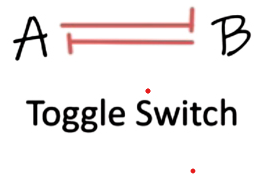
\includegraphics[width=20mm, scale=0.5]{toggle_switch_logo.png}
\end{figure}

\subsubsection*{Process Topology Information:} This process builds 
the ODEs based on the circuit topology (input). As an example the above circuit 
will be represented as 
\begin{align}
  \frac{dA}{dt} &= G_A H^S (B, B_A^0, n_{BA}, \lambda^{-}_{BA}) - k_A A \notag \\
  \frac{dB}{dt} &= G_B H^S (A, A_B^0, n_{AB}, \lambda^{-}_{AB}) - k_B B \notag 
\end{align}
Where, $A$ and $B$ represents the concentration of the protein $A$ and $B$ as  
a function of time, $G_A$ and $G_B$ are the maximum production rate of $A$ and 
$B$. $k_A$ and $k_B$ are the innate degradatino rates of the the corresponding 
proteins, and $H^S$ is non-linear shifted Hill function defined as
\begin{align}
  H^S (B, B_A^0, n_{BA}, \lambda^{-}_{BA}) & \coloneqq  \lambda^{-}_{BA} +
   \frac{1 -\lambda^{-}_{BA}}{1 + \left( \frac{B}{B_A^0}\right)^{n_{BA}}}
   \notag
\end{align} 
$\lambda^{-}_{BA}$ is the maximum fold change of A caused by inhibitor B. 

When multiple regulators target a gene, the function form of the rate equations 
assumes that these regulators are independent and hence, the overall production
rate becomes the product of the innate production rate of the target genes and 
the shifted Hill functions for all the regulatory links. 

\subsubsection*{Estimatation of parameters:}
Ranges of the threshold values in the shifted Hill functions are estimated 
numerically to satisfy the ``half-functoinal'' rule. Most of the other 
parametes are preset and sampled via a random distribution (which is `uniform 
distribution' by default). All these parameters are stored in a `.prs' (parameter)
file (e.g. ``circuit.prs'').

\subsubsection*{Solve the ODE, Identify the stable steady states:} RACIPE 
repeats the simulates teh coupled ODEs numerically for each sampled parameter
set for a large number of random initial conditions (optional input to RACIPE) 
and the steady state solutions for eac parameter set are stored in the output 
solution files.  
% ************************************************************************* %
%                                  THE END                                  %
% ************************************************************************* %
% ************************************************************************* %
%                                References                                 %
% ************************************************************************* %
\bibliography{citation} 
\bibliographystyle{abbrv}
% ************************************************************************* %  
\end{document} 